\documentclass[10pt,aspectratio=169]{beamer}
\usetheme{Madrid}
\usecolortheme{seahorse}
\usepackage[utf8]{inputenc}
\usepackage[T1]{fontenc}
\usepackage[french]{babel}
\usepackage{amsmath,amssymb,bm}
\usepackage{booktabs}
\usepackage{graphicx}

\newcommand{\T}[1]{\bm{\mathcal{#1}}}
\newcommand{\M}[1]{\bm{#1}}

\title[Modèles linéaires Tucker]{Fusion S2/S3 — Modèles linéaires de Tucker
couplée à c\oe ur parcimonieux}
\subtitle{Un modèle, cinq solveurs : ce que l'optimiseur change}
\author{Hamza BOUDA}
\institute{LISIC — ULCO \\ Point hebdomadaire d'équipe}
\date{16 juillet 2026}

\begin{document}

\begin{frame}
  \titlepage
\end{frame}

% ──────────────────────────────────────────────────────────
\begin{frame}{Contexte et objectif de la semaine}
\begin{columns}
\column{0.55\textwidth}
\textbf{Problème} : reconstruire la scène super-résolue
$\T{S}\in\mathbb{R}^{H\times W\times C}$ depuis
\begin{itemize}
  \item MSI fine spatialement ($c \ll C$ bandes) — rôle de S2 ;
  \item HSI grossière (ratio $r$) — rôle de S3.
\end{itemize}
\medskip
\textbf{Cette semaine} : consolider la \alert{famille linéaire} —
même modèle de Tucker couplé sparse, \alert{cinq algorithmes de résolution}
— avant le passage au non-linéaire.
\column{0.42\textwidth}
\textbf{Pourquoi ?}
\begin{itemize}
  \item baseline honnête pour l'article ;
  \item séparer \emph{effet du modèle} et \emph{effet du solveur} ;
  \item activer réellement la parcimonie du c\oe ur (demande centrale
        du sujet).
\end{itemize}
\end{columns}
\end{frame}

% ──────────────────────────────────────────────────────────
\begin{frame}{Le modèle (commun aux cinq architectures)}
Décomposition de Tucker couplée, c\oe ur parcimonieux :
\begin{equation*}
  \T{S} = \T{G}\times_1\M{D}_1\times_2\M{D}_2\times_3\M{D}_3
\end{equation*}
\begin{equation*}
\boxed{
  \min\;
  \lambda_H\bigl\lVert\T{H} - \T{S}\times_1\M{B}_h\times_2\M{B}_w\bigr\rVert_F^2
  + \lambda_M\bigl\lVert\T{M} - \T{S}\times_3\M{R}\bigr\rVert_F^2
  + \beta\lVert\T{G}\rVert_1}
\end{equation*}
\begin{itemize}
  \item Attache HSI $\to$ ancre les \textbf{spectres} ;
        attache MSI $\to$ ancre la \textbf{géométrie fine} ;
  \item $\ell_1$ sur $\T{G}$ : peu d'interactions triples
        (motif ligne $\times$ motif colonne $\times$ signature) ;
  \item Normalisation des colonnes de $\M{D}_n$ = lève l'ambiguïté
        d'échelle, $\beta$ garde un sens ;
  \item Initialisation SVD depuis les observations (jamais la référence).
\end{itemize}
\medskip
\textbf{vs prédécesseurs (G-STEREO)} : CPD de rang $F$, coût sans
$\ell_1$ — notre apport : structure Tucker \alert{+} parcimonie explicite
du c\oe ur.
\end{frame}

% ──────────────────────────────────────────────────────────
\begin{frame}{Cinq solveurs pour le même programme}
\centering
\small
\begin{tabular}{@{}lcccc@{}}
\toprule
 & Mise à jour & Pas & Zéros exacts & Coût/itér. \\
\midrule
ALS+FISTA   & alternée exacte & Lipschitz calculé & oui (prox) & élevé \\
Adam+prox   & simultanée & adaptatif/coordonnée & oui (prox) & faible \\
Adam+$\ell_1$ & simultanée & adaptatif/coordonnée & \alert{non} & faible \\
SGD+prox    & simultanée & global fixe & oui (prox) & faible \\
LBFGS+prox  & simultanée & courbure ($m{=}10$) & oui (prox) & $\sim$20$\times$ \\
\bottomrule
\end{tabular}
\medskip
\begin{itemize}
  \item Schéma \textbf{prox} : seuillage doux
        $\mathrm{S}_\tau(x)=\mathrm{sign}(x)\max(|x|-\tau,0)$ après chaque
        pas — \alert{vrais zéros} dans $\T{G}$ ;
  \item Schéma \textbf{pénalité} : $\beta\,\mathrm{sign}(\T{G})$ dans le
        gradient — rétrécit sans jamais annuler ;
  \item Protocole identique pour tous : mêmes opérateurs PSF/SRF,
        même init, mêmes 6 cas (3 PSF $\times$ ratios 4/8, bruit 35/30 dB).
\end{itemize}
\end{frame}

% ──────────────────────────────────────────────────────────
\begin{frame}{Résultats — 4 métriques, 2 scènes}
\centering
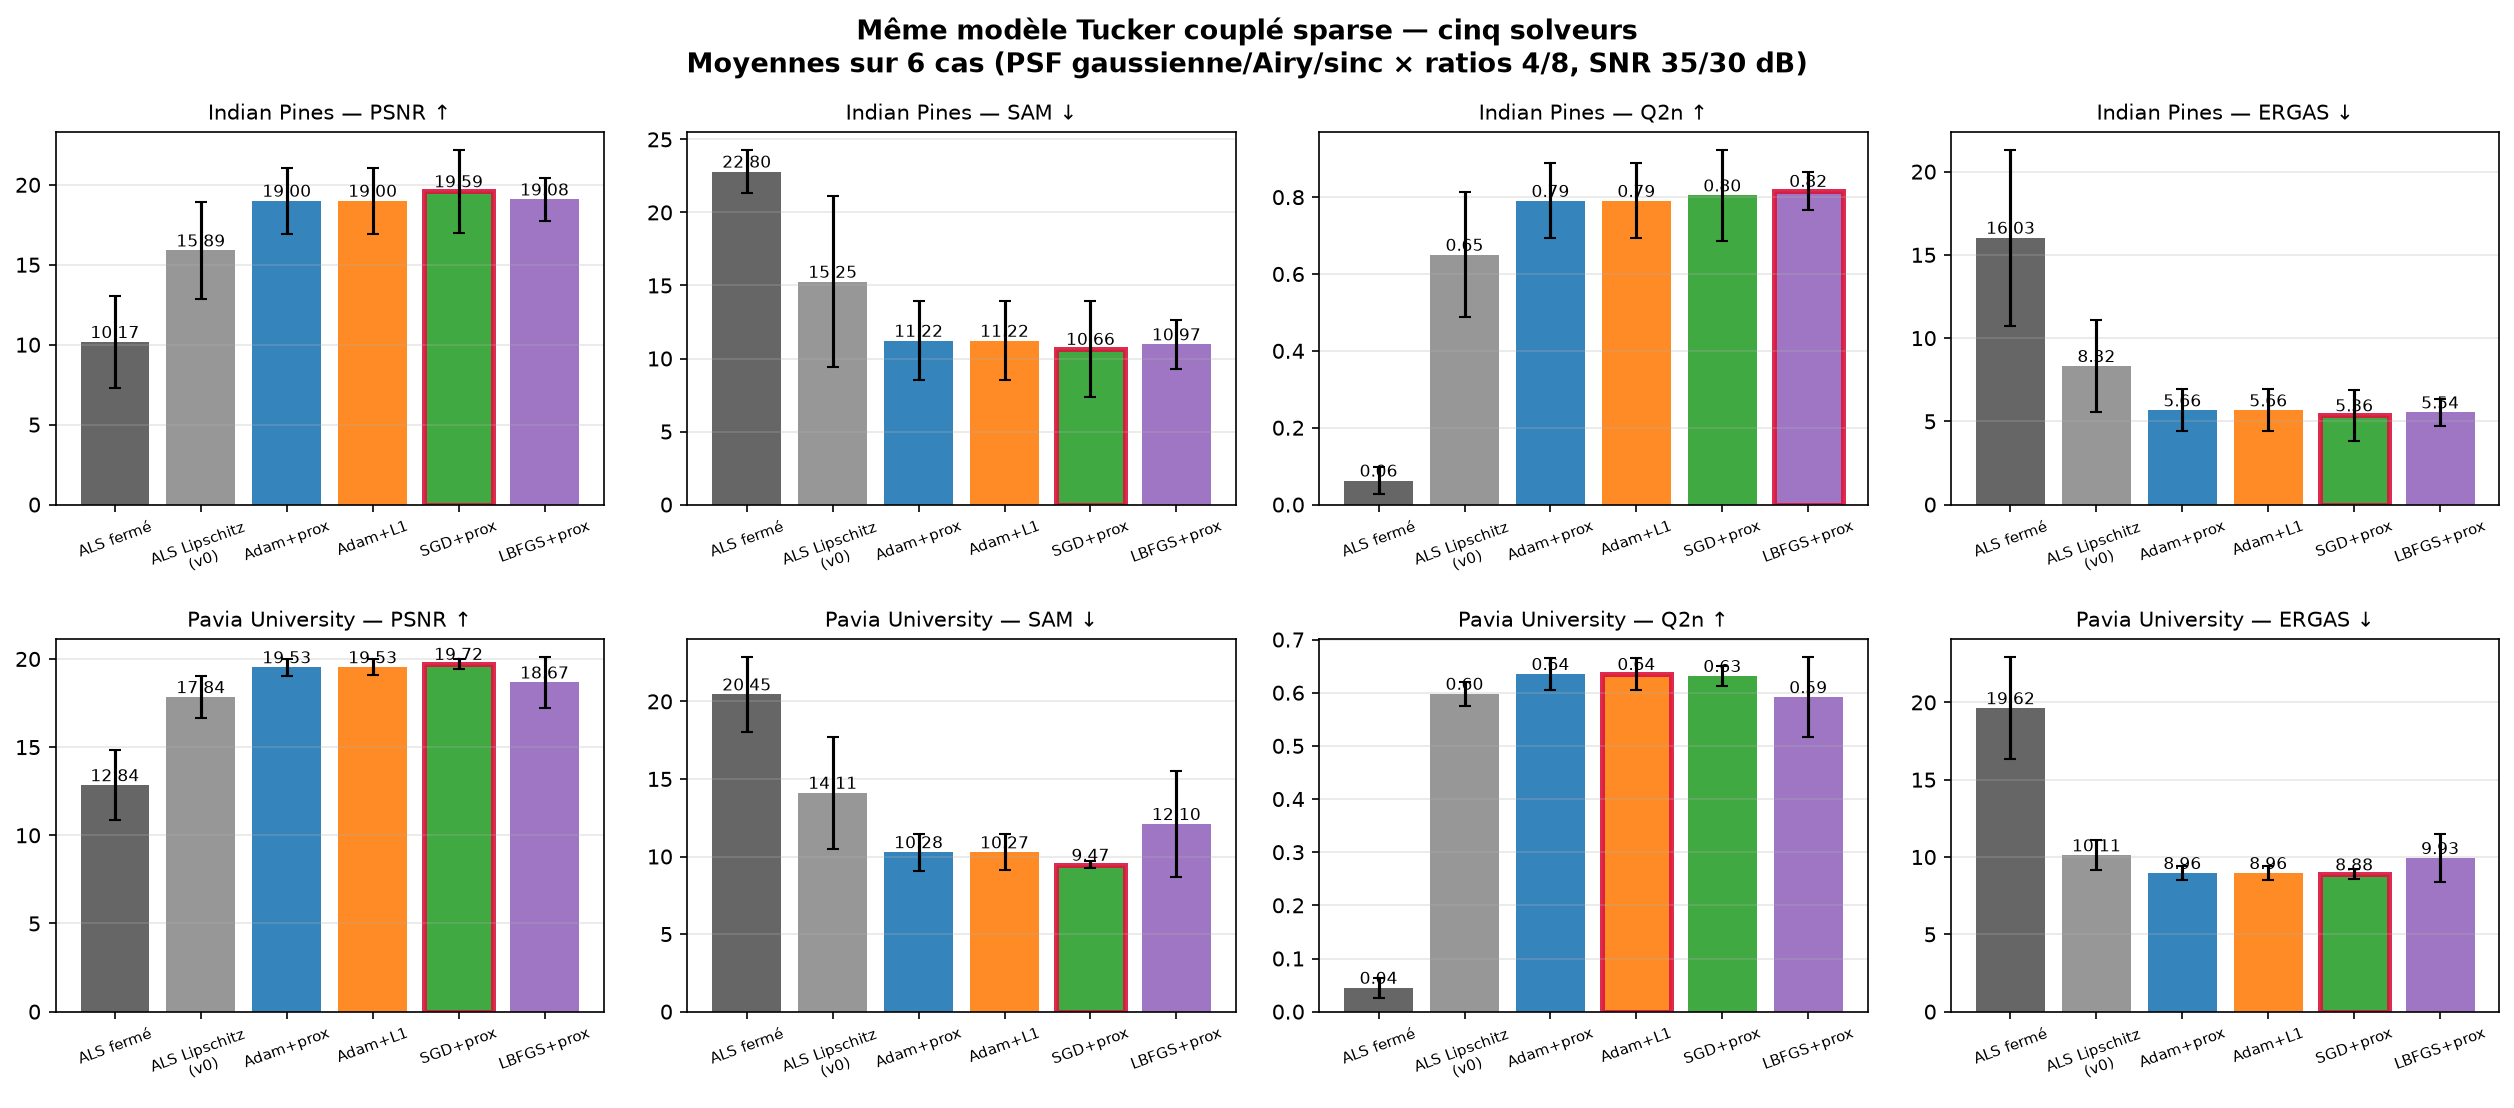
\includegraphics[width=0.98\textwidth]{figP1_metrics.png}
\end{frame}

% ──────────────────────────────────────────────────────────
\begin{frame}{Tableau récapitulatif}
\centering
\begin{tabular}{@{}lcccc@{\hskip 18pt}cccc@{}}
\toprule
 & \multicolumn{4}{c}{\textbf{Indian Pines}} & \multicolumn{4}{c}{\textbf{Pavia}} \\
\cmidrule(lr){2-5}\cmidrule(lr){6-9}
\textbf{Méthode} & PSNR & SAM & Q2n & ERGAS & PSNR & SAM & Q2n & ERGAS \\
\midrule
ALS + FISTA (fermé) & 10.17 & 22.80 & 0.06 & 16.03 & 12.84 & 20.45 & 0.04 & 19.62 \\
ALS + FISTA (Lipschitz, v0) & 15.89 & 15.25 & 0.65 & 8.32 & 17.84 & 14.11 & 0.60 & 10.11 \\
Adam + prox & 19.00 & 11.22 & 0.79 & 5.66 & 19.53 & 10.28 & 0.64 & 8.96 \\
Adam + $\ell_1$ & 19.00 & 11.22 & 0.79 & 5.66 & 19.53 & 10.27 & \textbf{0.64} & 8.96 \\
SGD + prox & \textbf{19.59} & \textbf{10.66} & 0.80 & \textbf{5.36} & \textbf{19.72} & \textbf{9.47} & 0.63 & \textbf{8.88} \\
LBFGS + prox & 19.08 & 10.97 & \textbf{0.82} & 5.54 & 18.67 & 12.10 & 0.59 & 9.93 \\
\bottomrule
\end{tabular}
\bigskip
\begin{itemize}
  \item Moyennes sur les 6 cas du protocole (3 PSF $\times$ ratios 4/8,
        SNR 35/30\,dB), meilleur en \textbf{gras} ;
  \item Même format que le tableau des méthodes MATLAB de l'équipe —
        comparaison directe possible dès que le protocole sera aligné
        (paramètres demandés).
\end{itemize}
\end{frame}

% ──────────────────────────────────────────────────────────
\begin{frame}{Lecture des résultats}
\begin{enumerate}
  \item \textbf{Le solveur domine l'écart} — hiérarchie à trois niveaux,
        à modèle strictement identique : ALS à mise à jour fermée approchée
        ($\sim$12.8\,dB) $\ll$ ALS à pas de Lipschitz, v0
        ($\sim$17.8\,dB) $<$ famille gradient ($\sim$19.5--19.7\,dB).
        \alert{Le détail d'implémentation de la mise à jour des
        dictionnaires vaut +5\,dB} ; le passage au gradient simultané
        en vaut $\sim$2 de plus.
  \item \textbf{Hiérarchie stable sur les deux scènes} :
        ALS $\ll$ SGD $<$ LBFGS $\approx$ Adam. Le conditionnement du
        problème est essentiellement \emph{diagonal} (échelles par
        coordonnée) : Adam suffit, la courbure croisée de LBFGS
        n'apporte rien à budget égal.
  \item \textbf{Conséquence méthodologique} : comparer un modèle
        non-linéaire (entraîné par gradient) à un linéaire résolu par ALS
        \alert{surestime} l'apport de la non-linéarité. Notre tableau
        d'article reportera les deux baselines.
\end{enumerate}
\end{frame}

% ──────────────────────────────────────────────────────────
\begin{frame}{Dynamique d'optimisation}
\centering
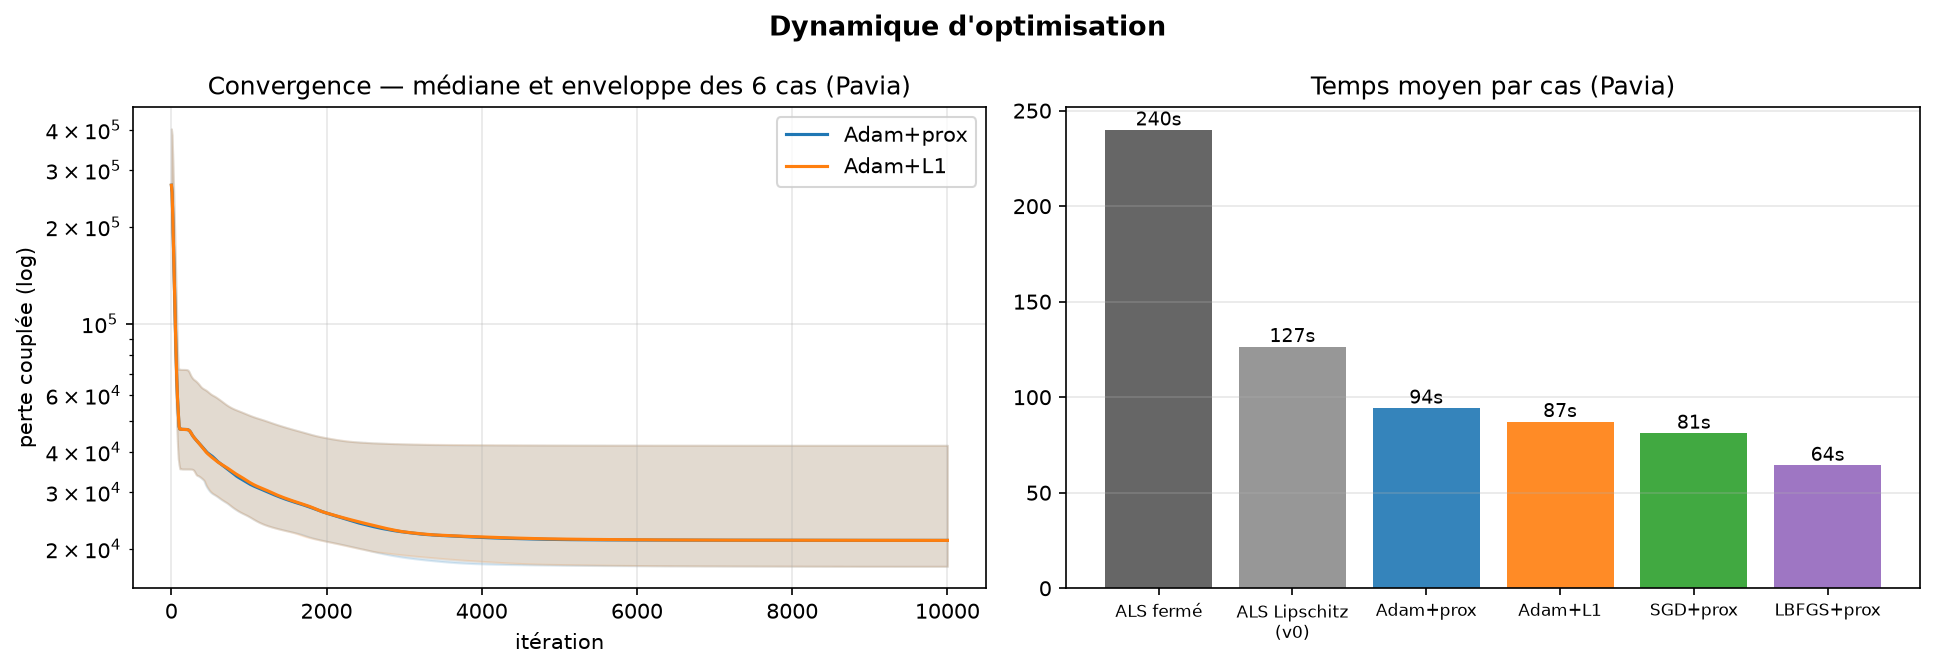
\includegraphics[width=0.95\textwidth]{figP2_convergence.png}
\begin{itemize}
  \item Deux phases : chute rapide ($\sim$150 itér., raffinement de
        l'init SVD) puis décroissance lente en loi de puissance ;
  \item Gradient : $\sim$40--90\,s par cas sur A100 — contre
        $\sim$4--5\,min pour l'ALS (CPU, systèmes linéaires + SVD).
\end{itemize}
\end{frame}

% ──────────────────────────────────────────────────────────
\begin{frame}{Parcimonie du c\oe ur : activer réellement le $\ell_1$}
\centering
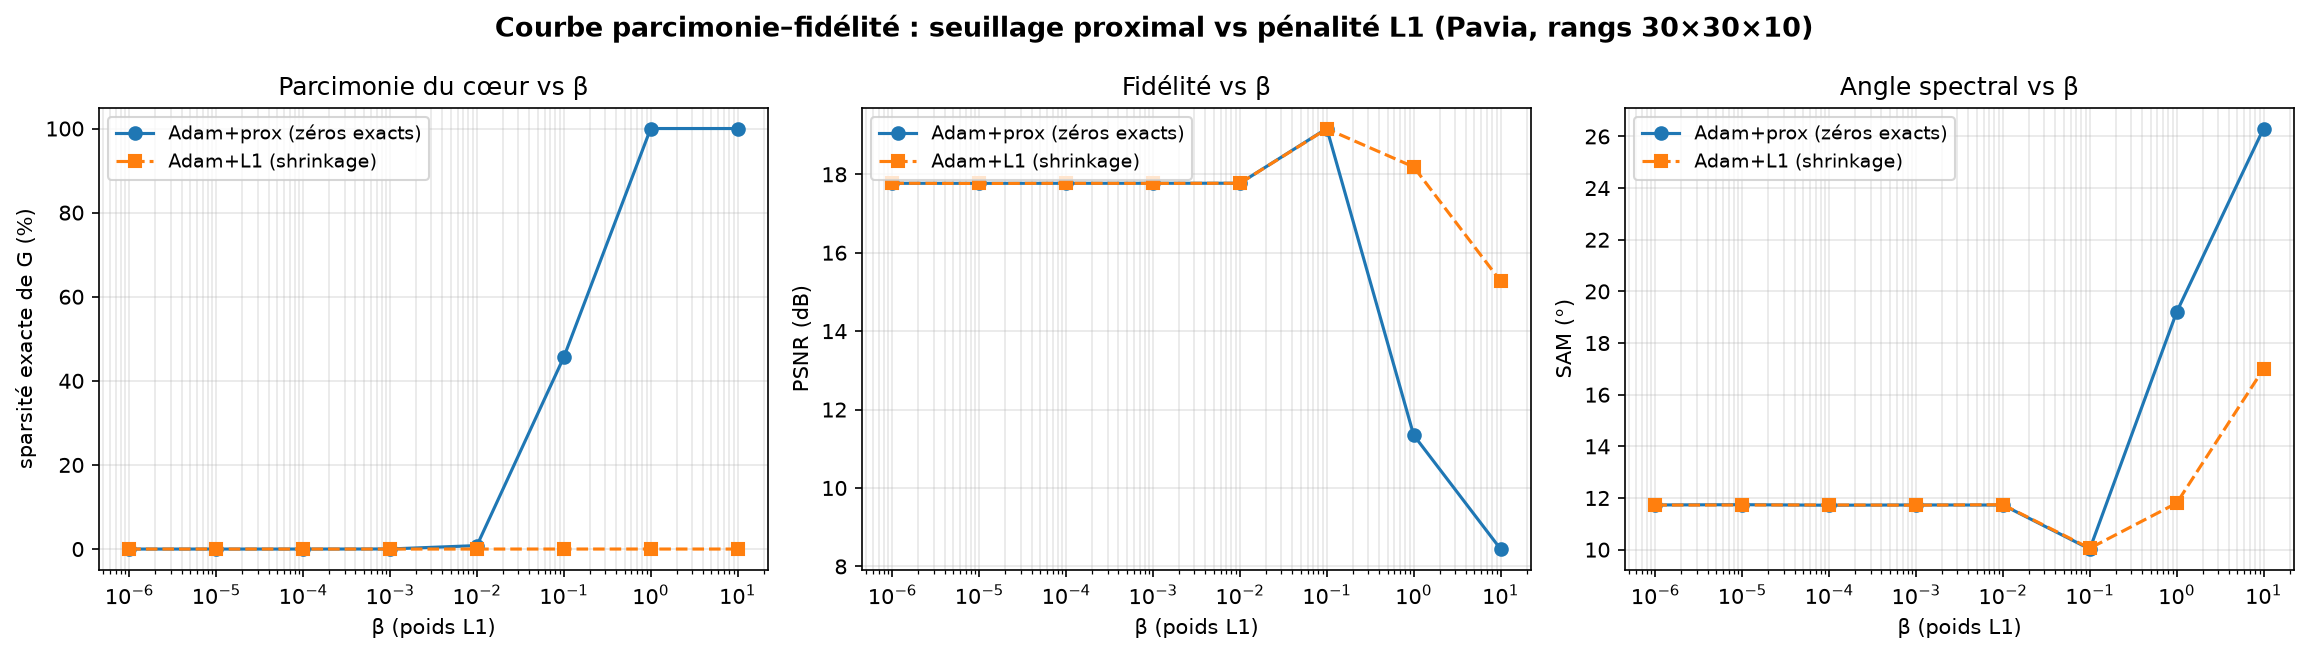
\includegraphics[width=0.98\textwidth]{figP3_sparsity.png}
\begin{itemize}
  \item Trois régimes : \textbf{inactif} ($\beta\le 10^{-2}$, sparsité
        $\approx$ 0), \textbf{utile} ($\beta \approx 0.1$),
        \textbf{mort du c\oe ur} ($\beta\ge 1$, 100\,\% de zéros,
        effondrement) ;
  \item \alert{Point clé : à $\beta=0.1$, un c\oe ur à 45\,\% de zéros
        exacts \emph{améliore} la fidélité (+1.4\,dB PSNR,
        $-1.7^\circ$ SAM)} — la parcimonie régularise, elle ne coûte pas ;
  \item Seul le schéma \textbf{proximal} atteint ce régime : la pénalité
        $\ell_1$ sous-différentiée rétrécit sans annuler
        (sparsité $= 0$ partout) et s'effondre plus tard mais sans
        interprétabilité.
\end{itemize}
\end{frame}

% ──────────────────────────────────────────────────────────
\begin{frame}{Conclusions des analyses}
\begin{enumerate}
  \item \textbf{Le solveur fait partie du modèle empirique} : à
        paramétrisation strictement identique, l'écart entre algorithmes
        d'optimisation atteint +7\,dB — plus que ce qu'apportent la
        plupart des changements de modèle. Toute comparaison de modèles
        doit donc fixer le cadre d'optimisation.
  \item \textbf{La famille gradient (Adam/SGD/LBFGS + prox) est le bon
        cadre} : meilleure fidélité sur toutes les métriques et les deux
        scènes, 3 à 10$\times$ plus rapide, et directement transposable
        au non-linéaire.
  \item \textbf{La parcimonie du c\oe ur est validée expérimentalement} :
        au bon réglage ($\beta \approx 0.1$), un c\oe ur à 45\,\% de zéros
        exacts \emph{améliore} la reconstruction (+1.4\,dB, $-1.7^\circ$
        SAM) — elle régularise, elle ne coûte pas. Seul le seuillage
        proximal atteint ce régime.
\end{enumerate}
\end{frame}

% ──────────────────────────────────────────────────────────
\begin{frame}{Prochaines étapes}
\begin{enumerate}
  \item \textbf{Réentraîner nos modèles dans les mêmes conditions
        d'entraînement que G-STEREO / STEREO / SCOTT} (même simulation
        des flux, mêmes opérateurs, mêmes métriques) pour une comparaison
        directe avec les méthodes de l'équipe ;
  \item \textbf{Sélectionner l'approche linéaire la plus performante}
        issue de cette étude (cadre gradient + seuillage proximal) ;
  \item \textbf{L'optimiser par grid search} : rangs $(R_1, R_2, R_3)$,
        poids de parcimonie $\beta$, taux d'apprentissage — avec un
        $\beta$ adaptatif à l'échelle du c\oe ur ;
  \item \textbf{Passer aux modèles non-linéaires (auto-encodeurs)} en
        réutilisant le même cadre : même perte couplée, mêmes opérateurs
        physiques, même seuillage proximal — seul le décodeur
        multilinéaire est remplacé par un décodeur appris.
\end{enumerate}
\end{frame}

\end{document}
